\subsection{Численные эксперименты}
Рассмотрим систему \eqref{cycle}, с параметрами \eqref{flow_exp1} (аналогичными эксперименту проточной цепи) и при этом
\begin{equation*}
    a_1 = 0.8, ~~ a_2 = 0.2, ~~ a_3 = 0.1. 
\end{equation*}
Имеем трофические цепи длиной от \(q=1\) до \(q=3\). При заданных значениях параметров имеем данные интервалы, ограничивающие поступление внешнего ресурса \(Q\):
\begin{enumerate}
    \item \( 0 < Q < 9.5 \);
    \item \( 9.5 < Q < 92.83\ldots \);
    \item \( 92.83\ldots < Q\).
\end{enumerate}
Аналогично, будем при разных значениях \(Q\) смотреть на графики с численностями и равновесными состояниями.

\begin{figure}[H]
    \centering
    \begin{subfigure}[t]{.45\linewidth}
        \centering
        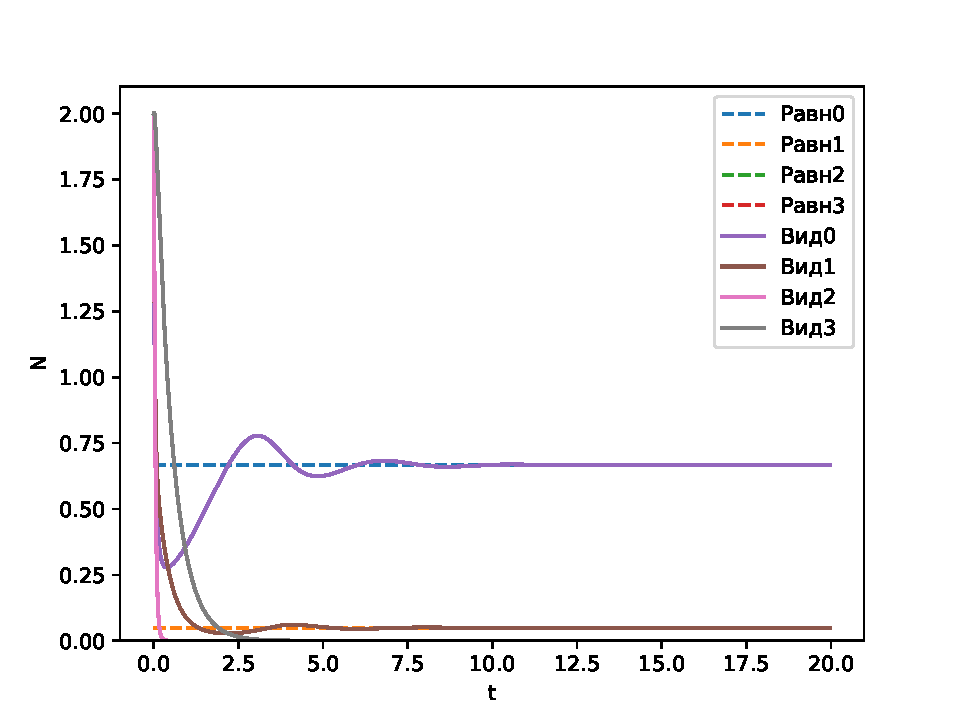
\includegraphics[width=\textwidth]{pictures/cycle/exp1_Q0.5.pdf}
        \caption{\(Q = 0.5\)}
    \end{subfigure}
    \begin{subfigure}[t]{.45\linewidth}
            \centering
            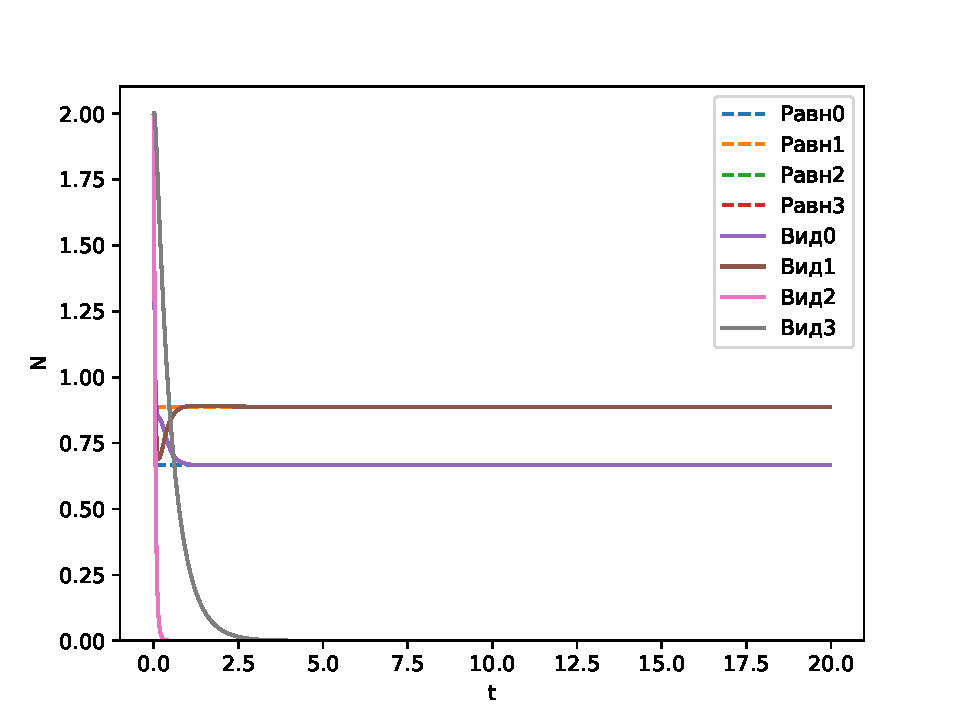
\includegraphics[width=\textwidth]{pictures/cycle/exp1_Q9.pdf}
            \caption{\(Q = 9\)}
        \end{subfigure}
    \caption{Численности видов системы, при \(Q\) близко к концам первого интервала.}  \label{fig:cycle_exp1_q1}
\end{figure}


\begin{figure}[H]
    \centering
    \begin{subfigure}[t]{.45\linewidth}
        \centering
        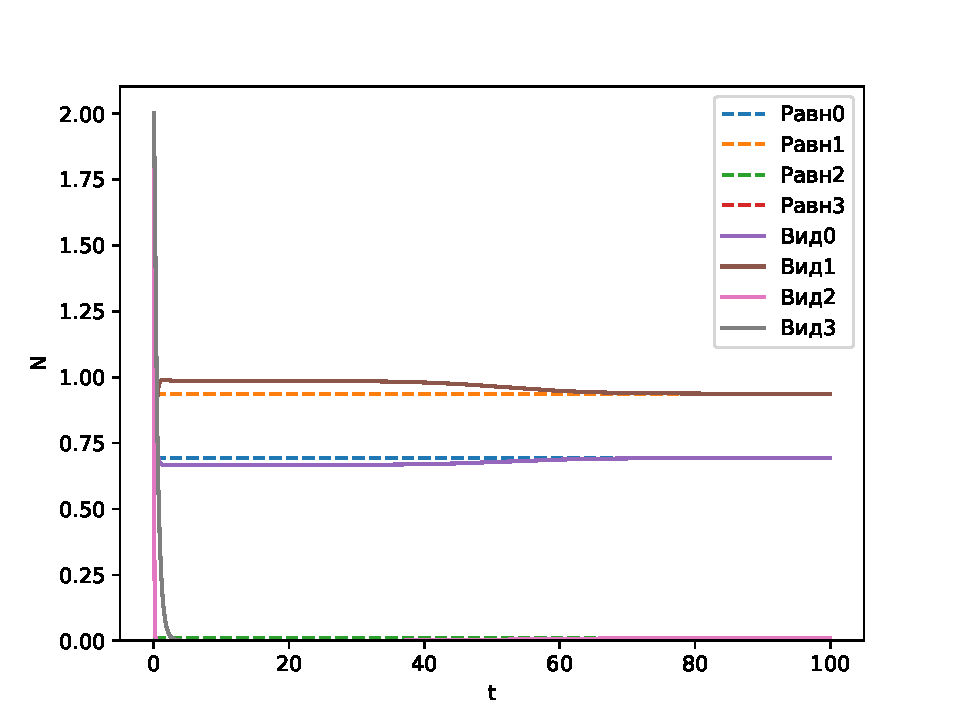
\includegraphics[width=\textwidth]{pictures/cycle/exp1_Q10.pdf}
        \caption{\(Q = 10\)}
    \end{subfigure}
    \begin{subfigure}[t]{.45\linewidth}
            \centering
            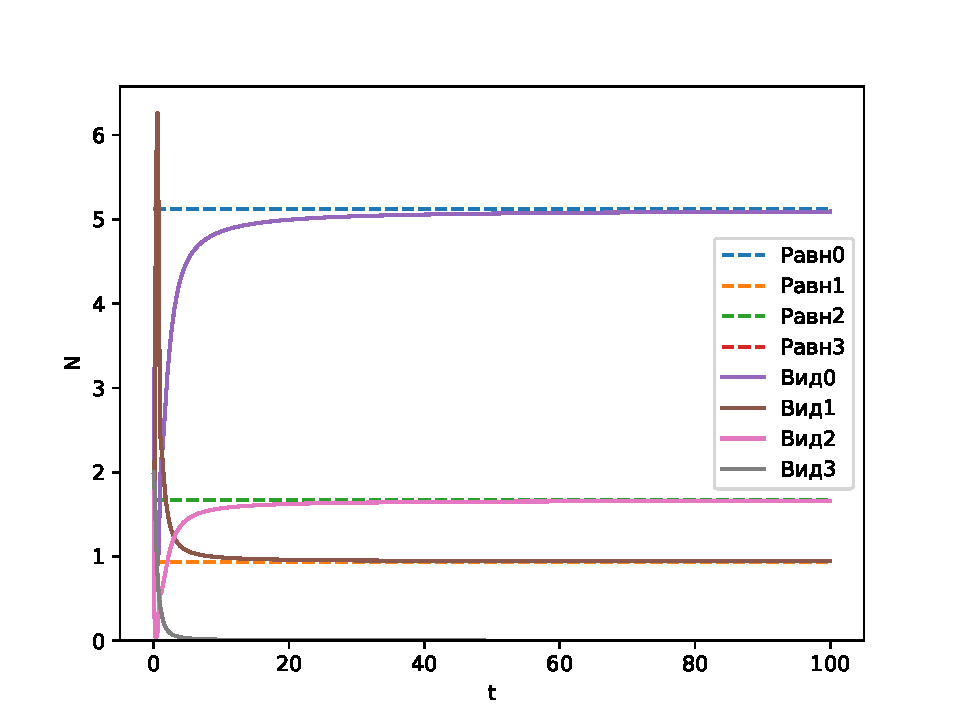
\includegraphics[width=\textwidth]{pictures/cycle/exp1_Q92.pdf}
            \caption{\(Q = 92\)}
        \end{subfigure}
    \caption{Численности видов системы, при \(Q\) близко к концам второго интервала.}  \label{fig:cycle_exp1_q2}
\end{figure}


\begin{figure}[H]
    \centering
    \begin{subfigure}[t]{.45\linewidth}
        \centering
        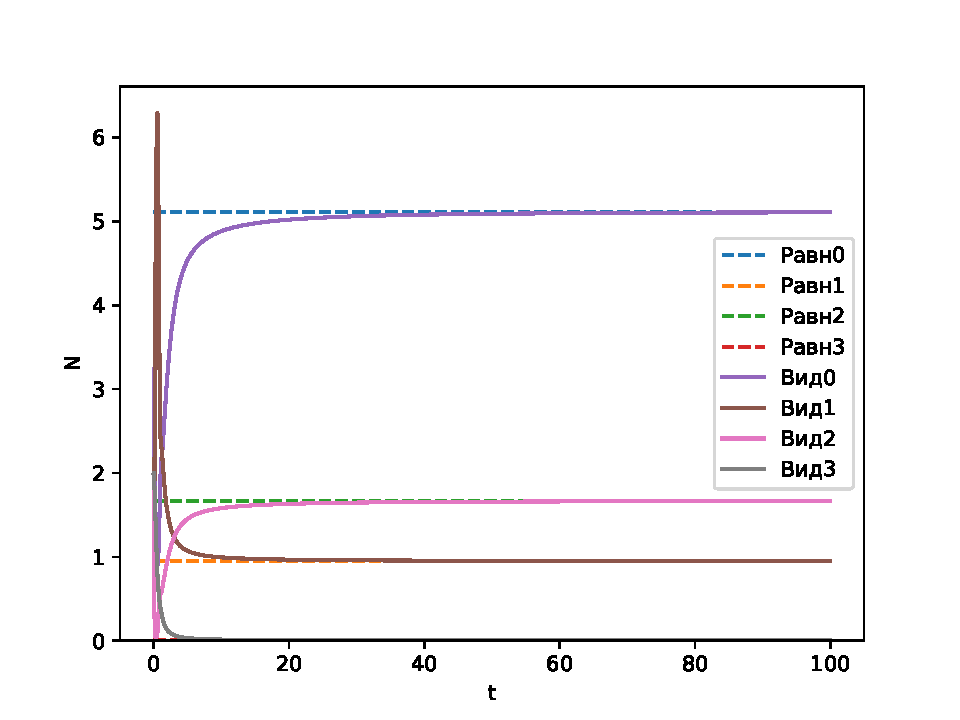
\includegraphics[width=\textwidth]{pictures/cycle/exp1_Q93.pdf}
        \caption{\(Q = 93, \quad N_3 \approx 0.0031\ldots \)}
    \end{subfigure}
    \begin{subfigure}[t]{.45\linewidth}
            \centering
            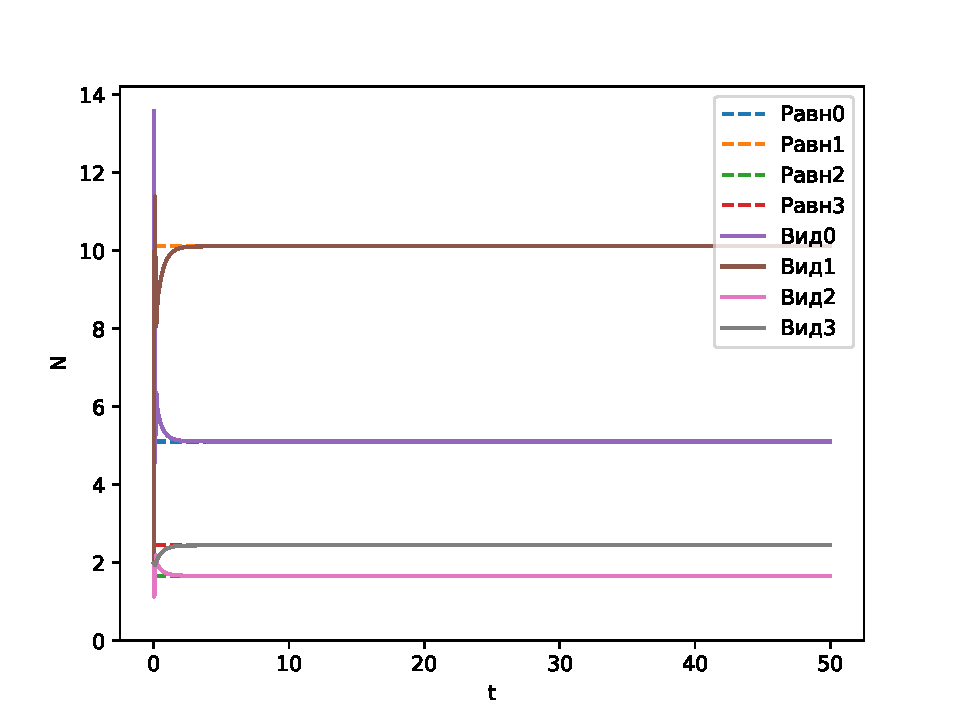
\includegraphics[width=\textwidth]{pictures/cycle/exp1_Q1000.pdf}
            \caption{\(Q = 1000\)}
        \end{subfigure}
    \caption{Численности видов системы, при \(Q\) близко к началу третьего интервала и на некотором отдалении.}  \label{fig:cycle_exp1_q3}
\end{figure}

Для небольшой модели из \(3\)-х видов отличия между проточной и циклической моделью небольшие. Эти обе модели ведут себя похоже и их основное отличие это разные интервалы устойчивости. 

Возьмём эту же модель, но при трофических функциях \( V_i(x) = \alpha_i \arctan x \).

\begin{figure}[H]
    \centering
    \subfigexp{0.5} {pictures/cycle/exp2_Q}{.3}
    \subfigexp{14}  {pictures/cycle/exp2_Q}{.3}
    \subfigexp{15}  {pictures/cycle/exp2_Q}{.3}
    \subfigexp{20}  {pictures/cycle/exp2_Q}{.3}
    \subfigexp{30}  {pictures/cycle/exp2_Q}{.3}
    \subfigexp{30.5}{pictures/cycle/exp2_Q}{.3}
    \subfigexp{40}  {pictures/cycle/exp2_Q}{.3}
    \subfigexp{100} {pictures/cycle/exp2_Q}{.3}
    \subfigexp{1000}{pictures/cycle/exp2_Q}{.3}
\caption{Численности видов системы.}  \label{fig:cycle_exp2}
\end{figure}

В сравнении с экспериментом на рис. \ref{fig:flow_exp2} данная модель при меньших значениях \(Q\) теряет асимптотическую устойчивость и становится периодической. 